\documentclass[tikz,border=2]{standalone}
\usepackage{amsmath}
\usepackage{pgfplots}
\usetikzlibrary{shapes,snakes,calc}
\tikzstyle{connector} = [->,thick]

\newsavebox\myboxa
\newsavebox\myboxb
\savebox\myboxa{%
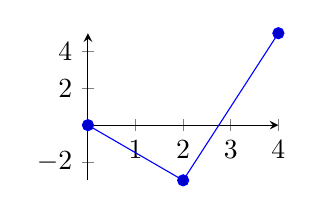
\begin{tikzpicture}
\begin{axis}[
  axis lines=middle,
  width=4cm,
]
\addplot coordinates {(0,0) (2,-3) (4,5)};
\end{axis}
\end{tikzpicture}%
}
\savebox\myboxb{%
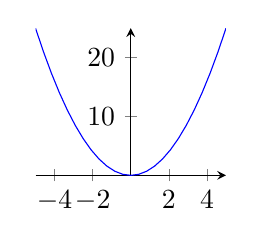
\begin{tikzpicture}
\begin{axis}[
  axis lines=middle,
  width=4cm
]
\addplot+[no marks] {x^2};
\end{axis}
\end{tikzpicture}%
}

\begin{document}

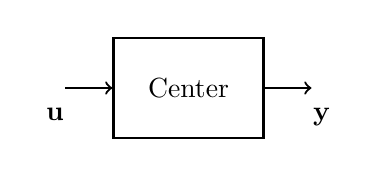
\begin{tikzpicture}[x=3in,y=2in]
    \tikzstyle{ann} = [draw=none,fill=none,right]
    \matrix[nodes={draw, thick, fill=none},
        row sep=0.3cm,column sep=0.5cm] {
    \node[draw=none,fill=none,label={below:$\mathbf{u}$}] (N1) {\usebox\myboxa}; &
    \node[rectangle, minimum height=0.5in, minimum width = 0.75in] (N2) {Center}; &
    \node[draw=none,label={below:$\mathbf{y}$}] (N3) {\usebox\myboxb};\\
    };

    \draw [connector] (N1) -- node {} (N2);
    \draw [connector] (N2) -- node {} (N3);
\end{tikzpicture}

\end{document}